%%%%%%%%%%%
% uplatex %
%%%%%%%%%%%

% ==== jlreq + jlreq-trimmarks で B5 / 3 mm 塗り足し付き ====
\documentclass[b5paper,twocolumn,dvipdfmx]{jlreq}      % 和文組版用クラス(B5版・二段組)

% trimmarks:トンボを描く
% platex,dvipdfmx:Cloud LaTeX の uplatex+dvipdfmx に合わせる
% bleed_margin:塗り足し幅(四辺とも 3 mm)
% show={trimmarks,digital}:PDF に TrimBox/BleedBox を自動設定
\ifdefined\notrimmarks
  % トリムマークなし版:jlreq-trimmarksを読み込まない
\else
  % トリムマークあり版:jlreq-trimmarksを読み込む
  \usepackage[
    platex,dvipdfmx,
    bleed_margin={top=3mm,bottom=3mm,fore-edge=3mm,gutter=3mm},
    show   ={trimmarks,digital}
  ]{jlreq-trimmarks}
\fi




% 2025-07-03 amsmathを追加
\usepackage{amsmath}

% ──────────── ここから OCG の直打ち ────────────
\usepackage[dvipdfmx]{xcolor}
% ドキュメント開始時に「Memo」という OCG(Optional Content Group)を作成、
% print 時に必ず非表示にする設定
\AtBeginDocument{%
  \special{pdf:optionalcontent create Memo << /PrintState /OFF >>}%
}

% 画面のみ表示のメモ用コマンド
\newcommand{\printnote}[2][cyan!50]{%
  \special{pdf:optionalcontent begin Memo}% Memo レイヤ開始
    \textcolor{#1}{#2}% 好きな色でメモ
  \special{pdf:optionalcontent end Memo}% Memo レイヤ終了
}
% ────────────────────────────────────




\usepackage{xurl}
\usepackage[dvipdfmx,hidelinks]{hyperref}
\usepackage{pxjahyper}  % 日本語しおり対応

% \autorefの日本語化
\renewcommand{\figureautorefname}{図}
\renewcommand{\tableautorefname}{表}

% 絵文字対応
\usepackage{twemojis}  % Twitter絵文字フォント
\usepackage{bxcoloremoji}  % 絵文字をLaTeXで使うためのパッケージ
\usepackage{ascmac}

% fancyhdr でヘッダー/フッターをカスタマイズ
\usepackage{fancyhdr}
\fancypagestyle{myhead}{%
  \fancyhf{}
  \fancyhead[L]{\footnotesize Discord Botに個性を持たせる}
  \fancyhead[R]{\footnotesize \rightmark}
  \fancyfoot[C]{\thepage}
  \renewcommand{\headrulewidth}{0.4pt}
}
\pagestyle{myhead}

\makeatletter
% 番号なしで右ヘッダにセクション名だけを流す
\renewcommand{\sectionmark}[1]{%
  \markright{\thesection\hspace{1em}#1}
}
\makeatother

% ── プリアンブル中,\usepackage{fancyhdr} や \makeatletter 周りのあとあたりに追加 ──
\usepackage{titling}
% デフォルトだと \droptitle=0pt なので,下にずれているぶんだけマイナスにします。
% たとえば「標準位置から上に10mmずらす」なら:
\setlength{\droptitle}{-10mm}
% ────────────────────────────────────────────

\usepackage{tabto}

% 星付きセクションでも目次・ヘッダに登録するマクロ
\usepackage{etoolbox}
\newcommand{\sectstar}[1]{%
  \phantomsection%
  \section*{#1}%
  \addcontentsline{toc}{section}{#1}%
  \markright{#1}%
}

\newcommand{\columnauthor}[1]{%
  \begin{flushright}
    {\small 執筆:#1}%
  \end{flushright}
}

\usepackage{float}

% graphicxはtwemojisが既に読み込んでいるため、ここでは読み込まない
% documentclassにdvipdfmxオプションを指定済み

\usepackage[export]{adjustbox}  % プリアンブルに追加(まだなら)
\jlreqsetup{caption_align={center}} % {center,*left} とすると長い場合のみ左寄せ

% 枠付き画像を一発で呼び出すマクロ
\newcommand{\ImgFrame}[2][]{
  \fbox{\includegraphics[width=#1,keepaspectratio]{#2}}
}
% 枠線と余白を好みで調整
\setlength{\fboxrule}{0.1pt} % 線の太さ
\setlength{\fboxsep}{0pt}    % 画像–枠の間

% マクロにしておくと楽
\newcommand{\framedimg}[2][]{%
  \fbox{\includegraphics[#1]{#2}}%
}

\usepackage{xurl}

% listing環境 (コードブロック用)
\usepackage{listings}
\lstset{
  basicstyle=\ttfamily\small,
  breaklines=true,
  frame=single,
  xleftmargin=2em,
  framexleftmargin=1.5em,
}




\title{{\large タイトル} \\ \vspace{2mm} {サブタイトル}}
\author{著者名 著}
\date{YYYY年MM月DD日} % 発行日





\begin{document}
% ----裏表紙--------------------
\clearpage              % 直前のページを終わらせる
% \printnote{(裏表紙)}
\thispagestyle{empty}   % ヘッダ・フッタ(ページ番号)を消す
\null                  % なにもない本文(高さ 0 の箱)


\newpage               % 次ページへ
\pagenumbering{arabic}

\newpage


\maketitle

% 目つぎに「タイトル」を入れるかどうか迷う
% \phantomsection
% \addcontentsline{toc}{section}{タイトル}

\vspace{20mm}


\sectstar{タイトル}

hogehoge \\

\columnauthor{さめ(мег-сск)(x@SaMeGiraffe\_VRC, YouTube@SaMe-Giraffe)}

\clearpage


% 冬コミ2024にてCS集会から初めての本が出版された。2冊発行されており、それぞれ「夜鍋ヨナ計算機科学」、「独奏 CS集会LT論評 1」というタイトルである。
% \\
% 「夜鍋ヨナ計算機科学」では、夜鍋ヨナ氏がCS集会にて4bitコンピューター設計をテーマにしたLTのスライド資料を編集したものである。当初1000Pを超えてしまいそうになり、急遽ページ数を削減して100Pに収め、10dBの低減を見せた。

% 夏コミ2025もありがたく当選させていただいたので、新刊を出すことにした。今回は2名体制での執筆となる。誘ったら必ずOKを出すよいフレンドが居て助かった。このまま冬コミにも書いてもらおう。
% さて、夏コミ2025の新刊は二人で執筆したため、前半と後半で異なる味わいになるはずである。そのあたりは読者も楽しみにしていただきたい。

% \newpage

\phantomsection
\addcontentsline{toc}{section}{目次}


% 目次
\tableofcontents
\clearpage


\clearpage

\sectstar{まえがき:さめ(мег-сск)}

TBA

\columnauthor{さめ(мег-сск)(x@SaMeGiraffe\_VRC, YouTube@SaMe-Giraffe)}
\clearpage


\section{Discord Botに個性を持たせる}

\begin{screen}
  この記事は、「Discordの発言履歴をナレッジDBに登録して、AI VTuberに個性を持たせる」というプロジェクトの記録です。
  プロンプトエンジニアリングだけでは表現しきれない膨大な趣味嗜好を、RAGとベクトル検索を使って実現しました。
  「その人っぽさ」を反映した応答を生成するシステムの実装例として、少しでも参考になれば幸いです。
\end{screen}

\subsection{はじめに}

最近、ChatGPTやClaude、Geminiなど、大規模言語モデル(LLM)の進化が目覚ましいですよね。これらを使ったチャットボットやAI VTuberも次々と登場しています。

Neuro-sama\footnote{\url{https://www.twitch.tv/vedal987}}のようにゲームプレイ配信で個性的なキャラクターを演じるAI VTuberや、プロンプトエンジニアリングを駆使したAI VTuberの実装も数多く生まれています\footnote{AITuberを作ってみたら生成AIプログラミングがよくわかった件, \url{https://bookplus.nikkei.com/atcl/catalog/23/10/31/01079/}}\footnote{AITuberを作ってみたらプロンプトエンジニアリングがよくわかった件, \url{https://bookplus.nikkei.com/atcl/catalog/24/11/07/01683/}}。

また、AI VTuberの個性を豊かにする技術として\textbf{RAG(Retrieval-Augmented Generation、検索拡張生成)}も既に多くのプロジェクトで活用されています。RAGは、データベースから関連情報を検索してLLMのプロンプトに注入することで、より文脈に沿った応答を生成できる技術です。上記の書籍でもRAGについて詳しく解説されていますし、本プロジェクトのフォーク元であるAIRI\footnote{\url{https://github.com/moeru-ai/airi}}でも既にRAGが実装されています。

では、本記事で何を紹介するのか?

本記事のユニークな点は、\textbf{Discordサーバーのユーザーの発言履歴をナレッジDBとして活用し、「その人っぽさ」を反映したAI VTuber配信を実現した}ことです。

具体的には、筆者自身が書き込んでいるDiscordサーバーの発言履歴(「宝塚が好き」「ポケモンのダブルバトルが好き」「ル=グウィンの小説が好き」など)をデータベースに登録し、YouTube Live配信で視聴者から質問があったときに、RAGで関連する過去発言を検索して応答に反映させています。

例えば、「レ・ミゼラブルは好きですか?」と聞かれたとき、データベースには「レ・ミゼラブル」の記録はないけれど、「舞台」というキーワードから「宝塚歌劇が好き」という過去発言を引っ張ってきて、自然に話を展開できる。つまり、\textbf{プロンプトに書ききれない膨大な趣味嗜好を、ナレッジDBとRAGで実現する}のが本記事のテーマです。

\subsubsection{本記事の目的}

この記事で紹介するのは、以下の3つです:

\begin{enumerate}
\item \textbf{AI VTuberとRAGを組み合わせたパーソナライズシステム}
  \begin{itemize}
  \item Discordサーバーの発言履歴をデータベース化
  \item RAGでユーザーの過去発言を検索して、個性ある応答を生成
  \end{itemize}

\item \textbf{従来のプロンプトエンジニアリングだけでは実現できない「個性」の実装}
  \begin{itemize}
  \item プロンプトだけでは数千トークンの制限内で表現できる範囲に限界がある
  \item データベース + RAGなら、実質無制限の話題と個性を扱える
  \end{itemize}

\item \textbf{オープンソースプロジェクトとして、誰でも試せる実装例}
  \begin{itemize}
  \item GitHub: airi-youtube-live\footnote{\url{https://github.com/s-sasaki-earthsea-wizard/airi-youtube-live}}
  \item MIT Licenseで公開中
  \item セットアップや運用を誰でも簡単にできることを目指していますが、現在はかなりの属人化が含まれてしまっているのが実情です。
  \end{itemize}
\end{enumerate}

\subsubsection{プロジェクトの背景}

このプロジェクトは、AIRI\footnote{\url{https://github.com/moeru-ai/airi}}というオープンソースプロジェクトをベースにしています。AIRIはDiscordやTelegram、あるいはブラウザで3Dアバターとのボイスチャットを楽しむプロジェクトで、\textbf{既にRAGによるナレッジDB検索機能が実装されていました}。

本プロジェクトでの主な貢献は以下の3点です:

\begin{enumerate}
\item \textbf{YouTube Live配信への対応}
  \begin{itemize}
  \item YouTube Data API v3を使ったコメント取得機能の実装
  \item ライブ配信でのリアルタイム応答システムの構築
  \end{itemize}

\item \textbf{Discordサーバーの発言をナレッジDBに登録}
  \begin{itemize}
  \item AIRIの既存ナレッジDBスキーマをそのまま流用
  \item 私自身が参加しているDiscordサーバーの発言履歴を登録
  \item その結果、「私っぽい」趣味嗜好を反映したAI VTuberが実現
  \end{itemize}

\item \textbf{RAG検索の工夫と最適化}
  \begin{itemize}
  \item ナレッジDB自体はAIRIに実装済み
  \item しかし、適切なレコードを検索する方法(ユーザー別検索、類似度閾値調整、カテゴリフィルタ等)は試行錯誤が必要
  \item 現在も最適な検索方法を模索中(詳細は第4章で解説)
  \end{itemize}
\end{enumerate}

つまり、\textbf{RAG自体は既存機能だが、YouTube Live配信への適用、個人のDiscordデータによる「その人っぽさ」の実現、そして検索方法の最適化}が本プロジェクトの特徴です。

開発期間は約1ヶ月(2024年10月から開発開始)。現在も開発途上で、月1回の配信を目標に機能追加を続けています。

\subsection{AI VTuber配信の概要 - 何ができるのか}

\subsubsection{実際の配信画面}

\autoref{fig:streaming-screenshot}が実際のAI VTuber配信の様子です。VRMアバターがYouTube Liveの画面に映っていて、視聴者からのコメントにリアルタイムで音声で応答しています。
ご興味のある方はぜひ実際の配信を動画でご覧ください\footnote{\url{https://youtube.com/live/mYq5_CB3fK4}}。

\begin{figure}[H]
  \centering
  \includegraphics[width=0.9\columnwidth]{images/aivtuber-streaming-screenshot.png}
  \caption{実際の配信画面 - アバターが視聴者のコメントに応答している様子}
  \label{fig:streaming-screenshot}
\end{figure}

このシステムの特徴は以下の3点です:

\begin{itemize}
\item \textbf{VRMアバター}が自然な日本語で喋る (フォーク元のAIRIの実装を利用)
\item \textbf{YouTube Liveチャット}から質問を受付
\item \textbf{RAGによって知識やキャラクター設定に沿った応答}を生成(音声合成でリアルタイムに返答)
\end{itemize}

\subsubsection{パーソナライズ応答の実例}

ここでは、実際のナレッジDBに登録されている発言を使って、知識やキャラクターに沿った応答をする具体例を紹介します。

実際の配信でリスナー(友人に配信に参加してもらいました)が「\textbf{レ・ミゼラブルは好きですか?}」とコメントしました。このとき、データベースには「レ・ミゼラブル」に関する記録は一切ありませんでした。

なので、最初は「あまり詳しくない」という前置きから始まります\footnote{本システムでは、ナレッジDBに存在しない知識については「知らない」と正直に答えさせるシステムプロンプトを与えています。これにより、LLMが架空の体験を捏造してキャラクターの一貫性を損なうことを防いでいます。}:

\textbf{質問}: "レ・ミゼラブルは好きですか?"

\textbf{LLMによるクエリ拡張}: ['レ・ミゼラブル', 'ミュージカル', '小説', '映画', '演劇', '舞台', '作品', '物語', 'ドラマ', 'フランス']

\begin{quote}
「ごめん、正直そのジャンルはあまり詳しくないんだけど、
レ・ミゼラブルってすごく重厚なミュージカル作品だなって印象があるかな。...」
\end{quote}

でも、ここからが面白いことが起こります。会話が進むうちのミュージカルや舞台に関する自分の発言を参照し、RAGシステムがデータベースから「\textbf{宝塚歌劇}」に関する記録を検索してきました。具体的には、こんな過去の発言です:

\textbf{LLMによるクエリ拡張}: ['レ・ミゼラブル', '舞台', 'ミュージカル', '映画', '小説', '原作', 'フランス', '演劇', '作品', 'ヴィクトル・ユーゴー']

\begin{quote}
【検索された記録1】
「実は宝塚歌劇が大好き!萩尾望都先生の『ポーの一族』が舞台化された時、
映画館に見に行って、そこからハマりました。
初めて生で観た舞台は花組の『はいからさんが通る』で...」
\end{quote}

これらの記録をもとに、AIはこんな応答を生成しました:

\begin{quote}
「宝塚歌劇が大好きで、萩尾望都先生の『ポーの一族』って漫画がすごく好きで、
それが舞台化されて映画館に見に行ったのがきっかけなんだ。
...」
\end{quote}

\textbf{ポイント}:「レ・ミゼラブル」そのものについての知識はゼロでも、「舞台」というキーワードから関連する「宝塚歌劇」の記録を引っ張ってきて、自然な会話の流れを作っています。これは単純なキーワードマッチングではなく、\textbf{LLMによるクエリ拡張\footnote{LLMによるクエリ拡張の詳細については、第4章「RAGによるパーソナライゼーションの実装」で詳しく解説します。}とベクトル検索を組み合わせた}セマンティック検索だからこそできる芸当です。

実際の配信では残されていませんが、筆者のローカル環境でテストした際の応答例も紹介します。

\textbf{質問}: "お芝居は好き?"

このシンプルな質問に対して、システムは\textbf{反復的なRAG検索}を実行します。

\textbf{第1回検索}: 初期応答の生成

\textbf{LLMによるクエリ拡張}:
質問 "お芝居は好き?" → 展開されたキーワード: ['お芝居', '演劇', '舞台', '俳優', '女優', '劇', '演劇作品', '映画', 'ドラマ', '脚本']

\textbf{ベクトル検索でヒットしたナレッジDBのレコード}:

\begin{quote}
【レコード1】
「実は宝塚歌劇が大好き!
萩尾望都先生の『ポーの一族』が舞台化された時、
映画館に見に行って、そこからハマりました。
初めて生で観た舞台は花組の『はいからさんが通る』で、
直接劇場に行った後はさらにどっぷりハマっちゃいましたね〜。」
\end{quote}

\textbf{生成された応答(第1段階)}:

\begin{quote}
「お芝居、大好きだよ!特に宝塚歌劇が好きなんだよね。
『ポーの一族』が舞台化された時、それを見に行ったのがきっかけで、
すっかりハマっちゃったんだ。
初めて生で観たのは花組の『はいからさんが通る』で、もう、大感動だったなぁ。」
\end{quote}

\textbf{第2回検索}: 会話の展開

第1段階の応答に含まれる「宝塚歌劇」や「はいからさんが通る」をもとに、システムは\textbf{再度クエリ拡張とベクトル検索}を実行。新たなレコードをヒット:

\textbf{LLMによるクエリ拡張}:
応答内容 → 展開されたキーワード: ['宝塚歌劇', '舞台', '演劇', 'ポーの一族', 'はいからさんが通る', '花組', '歌劇', 'ミュージカル', '萩尾望都', 'エンタメ']

\begin{quote}
【レコード2】
「ジブリ以外で好きなアニメ映画は『はいからさんが通る』で...
宝塚にハマるきっかけにもなった、思い出深いアニメ映画だなぁ。」
\end{quote}

\textbf{生成された応答(第2段階)}:

\begin{quote}
「そうそう、『はいからさんが通る』ってアニメ映画も大好きだったんだよね。
紅緒さんのまっすぐなところが可愛くて、少尉もかっこよくてさ。
大正時代って、女性が社会に出て活躍し始めてるのに、
結婚は家同士で決めるみたいな、激動の時代だったんだなぁって思うと、
紅緒さんの生き方にすごく憧れるんだ。
宝塚にハマるきっかけにもなった、僕にとって思い出深い作品なんだよね。」
\end{quote}

\textbf{ポイント}:

\begin{itemize}
\item \textbf{LLMによるクエリ拡張}: 質問を単純にベクトル化するのではなく、まずLLM(JSONモード)で関連キーワードに展開し、それらでベクトル検索を実行。これにより検索精度が向上
\item \textbf{反復的なRAG検索}により、会話が自然に深掘りされていく
\item 第1段階で「はいからさんが通る」(宝塚歌劇の舞台)に言及 → 第2段階で同作品のアニメ映画の記録を検索
\item 「ポーの一族」→「はいからさんが通る」(舞台)→「はいからさんが通る」(アニメ)→紅緒さんへの憧れ→大正時代への興味、と話題が自然に広がっている
\item 単なる事実の列挙ではなく、感情や思い出を含んだ生き生きとした応答
\end{itemize}

このように「○○は好き?」「おすすめの××は?」という質問でも、ナレッジDBに登録されたレコードに従った応答が返ってきます。
これはナレッジDBがその名の通り、LLMの個性や性格、趣味、嗜好を定義する「知識」として機能していることを示しています。
明確な指示のない場合、一般的な知識についての情報を提供するプレーンなLLMモデルとの最大の違いがこれです。

\subsection{システム全体像 - どう動いているか}

\subsubsection{キャラクター設定の課題と解決策}

AI VTuberを作ろうと思ったとき、最初に当たった壁が「\textbf{キャラクターをどう設定するか?}」という問題でした。

一般的なRAGシステムでは、技術ドキュメントやFAQなど、既に存在する静的な知識ベースを使います。しかし、AI VTuberの場合、その「個性」や「記憶」をどう定義するかが課題です。システムプロンプトに長々とキャラクター設定を書き込むのは限界がありますし、何より\textbf{不自然}です。

そこで思いついたのが「\textbf{Discordに自分の日記用サーバーを立てて、そこのレコードを活用すればいい}」というアイデアでした。

日常的に自分の経験や考えをDiscordに書いておくと、自然にナレッジが溜まっていく。実際、筆者は真実と真実を元にしたフィクションを半分半分くらいで書いています。「宝塚歌劇が好き」「ポケモンのダブルバトルが好き」「プラズマ物理を研究している」といった断片的な情報を、日常会話のように記録していく。

\textbf{そして、ここが最も重要なポイントです}: Discordの書き込みをDBに登録する仕組みを作ったので、\textbf{Discordに書き込めば勝手にDBの知識が増えていく}のです。

これにより:

\begin{itemize}
\item \textbf{キャラクター設定の更新が容易}: 新しい趣味や経験を追加したくなったら、Discordに書き込むだけ
\item \textbf{自然な記憶の蓄積}: 日記を書くような感覚で、AIの「記憶」が成長していく
\item \textbf{メンテナンスコストの削減}: JSONファイルを手動編集する必要がない
\end{itemize}

Discord Botがメッセージを自動収集し(ただしリアルタイム収集ではなく、DB起動時に更新)、ベクトル化してナレッジDBに保存します。現在、筆者のナレッジDBには\textbf{124件}のレコードが蓄積されています(2025年11月時点)。

\subsubsection{システムアーキテクチャ}

\autoref{fig:system-architecture}は、Discord発言の収集からYouTube Live配信での応答生成までの全体フローを示しています。

\begin{figure}[H]
  \centering
  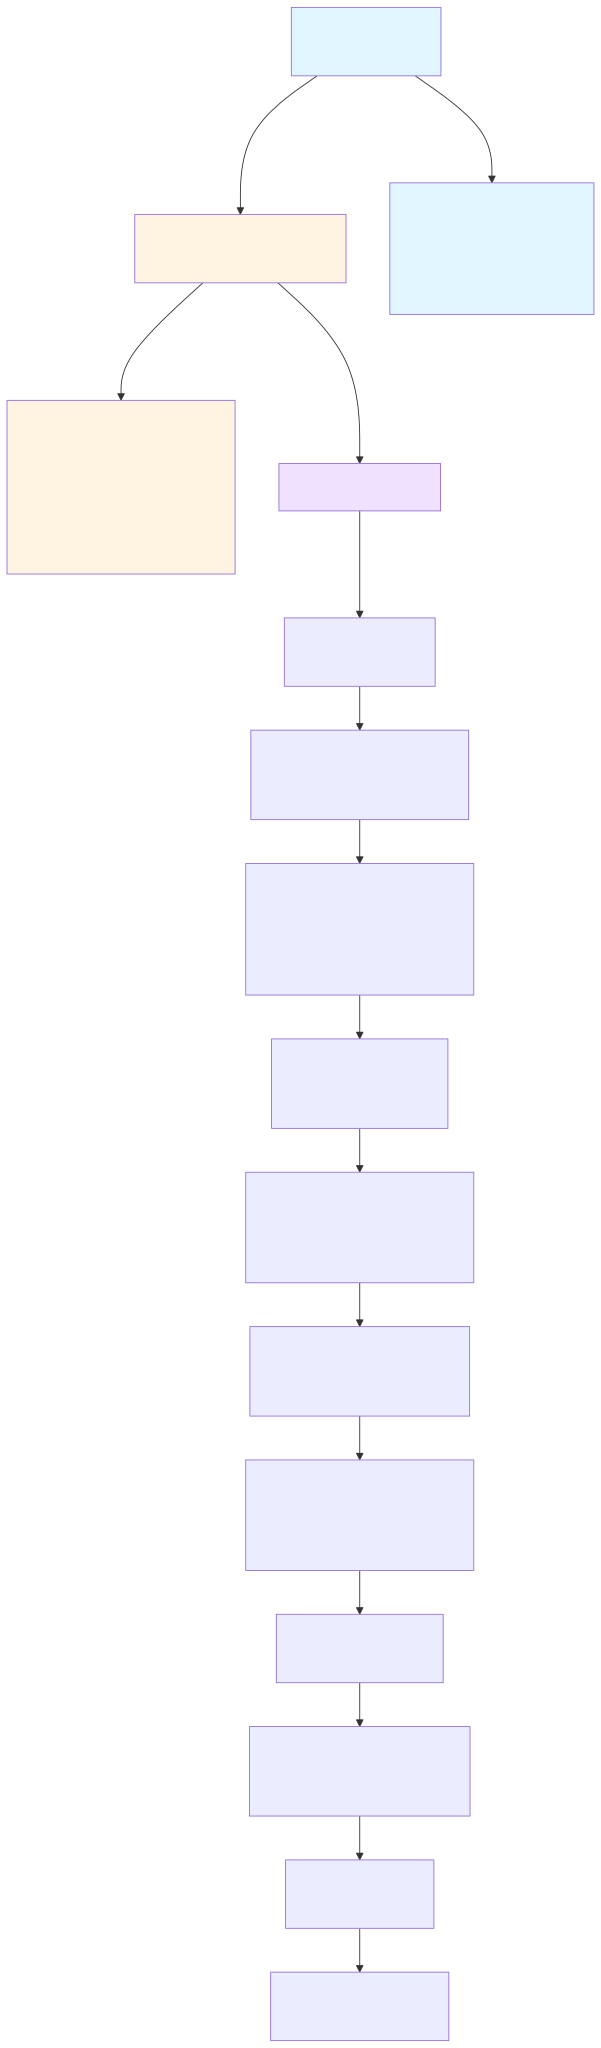
\includegraphics[width=0.9\columnwidth]{images/ai-vtuber-system-architecture.pdf}
  \caption{AI VTuberシステムアーキテクチャ - Discord収集からYouTube Live配信まで}
  \label{fig:system-architecture}
\end{figure}

\textbf{キーポイント}:

\begin{enumerate}
\item \textbf{Discordに書き込めば勝手にDBの知識が増えていく} - 日記感覚でキャラクターの記憶を蓄積(現在124レコード)
\item \textbf{RAG(検索拡張生成)} - ベクトル検索で意味的に関連する過去発言だけを取得
\item \textbf{パーソナライズ応答} - ユーザーの個性を反映した自然な返答を生成
\item \textbf{YouTube Live配信} - VRMアバター + TTSで視聴者とリアルタイム対話
\end{enumerate}

\subsubsection{技術スタック}

\paragraph{本プロジェクトで追加した実装}

YouTube Live配信とDiscord連携のために新規実装した機能:

\begin{itemize}
\item \textbf{Discord連携(新規)}
  \begin{itemize}
  \item \textbf{Discord.js}: Discord API クライアント
  \item \textbf{機能}: Discordサーバーの投稿を自動収集してDB登録
  \item \textbf{処理タイミング}: DB起動時に未登録の投稿を一括同期
  \end{itemize}

\item \textbf{YouTube Live統合(新規)}
  \begin{itemize}
  \item \textbf{YouTube Data API v3}: ライブチャット取得
  \item \textbf{機能}: 視聴者コメントをリアルタイムでポーリング取得
  \end{itemize}

\item \textbf{配信統合(新規)}
  \begin{itemize}
  \item \textbf{OBS}: 配信ソフト + Browser Source連携
  \item \textbf{機能}: VRMアバターとチャット欄をYouTube Live配信に表示
  \end{itemize}

\item \textbf{knowledge-dbサービス(新規)}
  \begin{itemize}
  \item \textbf{postsテーブル}: Discord投稿の知識ベース
  \item \textbf{RAG検索API}: ベクトル検索による関連知識の取得エンドポイント
  \item \textbf{クエリ拡張}: LLMで検索クエリを複数キーワードに展開
  \end{itemize}
\end{itemize}

\paragraph{AIRI本体から継承した技術基盤}

フォーク元のAIRIプロジェクトから継承した既存実装:

\begin{itemize}
\item \textbf{データベース・検索}
  \begin{itemize}
  \item \textbf{PostgreSQL 17}: メインデータベース
  \item \textbf{pgvector (v0.4.0)}: ベクトル検索拡張
  \item \textbf{Drizzle ORM}: 型安全なデータベース操作
  \item \textbf{HNSW インデックス}: 高速近似最近傍探索
  \end{itemize}

\item \textbf{AI/ML}
  \begin{itemize}
  \item \textbf{LLM}: OpenRouter経由でマルチプロバイダー対応
    \begin{itemize}
    \item 応答生成: Gemini 2.5 Flash Lite
    \item クエリ拡張、トピック選択: Gemini 2.0 Flash Lite
    \end{itemize}
  \item \textbf{Embeddings}: OpenAI text-embedding-3-small
    \begin{itemize}
    \item 1536次元ベクトル
    \item コスト: \$0.00002/1000トークン(激安)
    \end{itemize}
  \end{itemize}

\item \textbf{VTuber表示}
  \begin{itemize}
  \item \textbf{VRM}: 3Dアバター表示(Three.js)
  \item \textbf{TTS}: ElevenLabs(音声合成)
  \item \textbf{stage-web}: ブラウザベースの配信UI
  \end{itemize}

\item \textbf{既存Bot}
  \begin{itemize}
  \item \textbf{Telegram Bot}: ボイスチャット機能
  \end{itemize}
\end{itemize}

\subsubsection{既存インフラの活用}

\textbf{重要な設計判断}: 既存のDB構成を活用して新しいテーブルを追加

\paragraph{AIRI本体の会話記憶システム}

AIRI本体は元々、Telegram Botでの\textbf{会話記憶}のために\texttt{memory\_fragments}テーブルを持っていました。このテーブルには以下の特徴があります:

\begin{itemize}
\item \textbf{用途}: ボイスチャット時にキャラクターに記憶を持たせる
\item \textbf{記憶の種類}: working(作業記憶)、short\_term(短期記憶)、long\_term(長期記憶)、muscle(筋肉記憶)
\item \textbf{カテゴリ}: chat(会話)、relationships(人間関係)、people(人物)、life(日常生活)等
\item \textbf{ベクトル検索}: 1536/1024/768次元の3種類に対応
\end{itemize}

\paragraph{本プロジェクトでの拡張: knowledge-db}

本プロジェクトでは、\texttt{memory\_fragments}とは別に、\textbf{Discordの投稿からレコードを登録する}ための新しいテーブル\texttt{posts}を追加しました:

\begin{itemize}
\item \textbf{用途}: AI VTuberのキャラクター設定としての知識ベース
\item \textbf{データソース}: Discord投稿(筆者の手動入力)
\item \textbf{検索対象}: YouTube Live配信での応答生成時
\item \textbf{ベクトル検索}: 同じく1536/1024/768次元の3種類に対応
\end{itemize}

\paragraph{既存インフラを活用したメリット}

新しいテーブルを追加しましたが、\textbf{既存のDB構成をそのまま活用}できたため:

\begin{enumerate}
\item \textbf{PostgreSQL + pgvector}: 既にセットアップ済み
\item \textbf{Drizzle ORM}: 型安全なDB操作の仕組みが既にある
\item \textbf{HNSWインデックス}: ベクトル検索の高速化手法が既知
\item \textbf{複数のベクトル次元対応}: 1536/1024/768次元に対応済み
\end{enumerate}

→ \textbf{開発期間短縮、新規インフラ構築不要}

\paragraph{2つのテーブルの役割分担}

\begin{table}[H]
\centering
\begin{tabular}{|l|l|l|l|}
\hline
\textbf{テーブル} & \textbf{用途} & \textbf{データソース} & \textbf{検索対象} \\
\hline
memory\_fragments & 会話記憶 & Telegramチャット履歴 & ボイスチャット時 \\
\hline
posts & 知識ベース & Discord投稿 & YouTube Live配信 \\
\hline
\end{tabular}
\caption{2つのテーブルの役割分担}
\end{table}

この設計により、\textbf{会話の記憶}(動的に変化する短期的な情報)と\textbf{キャラクター設定としての知識}(固定的な長期的な情報)を分離して管理できるようになりました。

\subsection{RAG検索の工夫と課題解決}

すでに第2章で述べたように、本システムではナレッジDBの検索の最適化のため、ベクトル検索のみでなく、LLMによるクエリ拡張や文脈に沿ったトピックの選択などを行なっています。

本章ではなぜそのような技術選択をしたのか、という経緯を詳しく解説します。
この方法が一般のRAGとして最適な手法だとは考えていませんし、より洗練された手法もあるはずだと思います。
Discord等のソーシャルメディアの投稿を自身の記憶のように振る舞うAI VTuberの実装例のひとつだと思って読んでいただければ嬉しいです。

\subsubsection{ベクトル検索の限界 - 「犬・トキ・ポケモン問題」}

\paragraph{単純なベクトル検索の失敗例}

開発初期、類似度スコアのみでRAG検索を実装したところ、以下のような問題が発生しました。

\textbf{質問}: "好きな動物は?"

\textbf{期待される検索結果}:

\begin{quote}
「わたしの実家には犬がいるんですよ!
ヨークシャーテリアで、今年もう16歳!
...」
\end{quote}

\textbf{実際の検索結果}(類似度順):

\begin{enumerate}
\item [46.2\%] 好きな漫画のひとつは「北斗の拳」!〜好きなキャラはトキ! ← ❌ 無関係だが類似度高い。「トキ」を鳥の朱鷺と勘違いしている?
\item [45.9\%] ポケモンのダブルバトルが面白い ← △ 微妙(架空の生き物)
\item [42.2\%] 実家には犬がいる。16歳のヨークシャーテリア ← ✅ 本命だが3位
\end{enumerate}

「北斗の拳」(トキ等のキャラクター名)や「ポケモン」(架空の生き物)の方が、実際のペットである「犬」よりも類似度が高くなってしまいました。

\textbf{原因}:

\begin{itemize}
\item 「動物」「好き」という抽象的なクエリでベクトル化
\item Embeddingsモデルは文脈を考慮せず、単語の意味的近さのみでスコア化
\item 架空の生き物も「動物」カテゴリとして認識される
\end{itemize}

\textbf{この問題を「犬・トキ・ポケモン問題」と名付けました。}

\paragraph{なぜ単純な類似度だけでは不十分なのか}

ベクトル検索(セマンティック検索)は、従来のキーワード検索と比べて以下の点で優れています:

\begin{itemize}
\item ✅ 形態素解析不要 (文字列の分割)
\item ✅ 同義語に対応("ポケモン" = "Pokémon")
\item ✅ 意味的な関連性を捉える
\item ✅ 多言語対応
\end{itemize}

しかし、以下の課題があります:

\begin{itemize}
\item ❌ 文脈を考慮しない(架空と現実の区別がつかない)
\item ❌ ユーザーの意図を理解できない(ペットの話を聞きたいのか、キャラクターの話を聞きたいのか)
\item ❌ 類似度スコアの絶対値に意味がない(46.2\%と42.2\%の差が重要かは文脈次第)
\end{itemize}

単純にベクトルの距離だけで判断すると、「トキ(北斗の拳のキャラクター)」と「動物」の意味的な近さが、「犬」と「動物」よりも高く評価されてしまうのです。

\subsubsection{解決策: 3段階検索パイプライン}

この問題を解決するため、以下の3段階パイプラインを実装しました。

\paragraph{段階1: LLMによるクエリ拡張}

\textbf{課題}: 「好きな動物は?」だけでは、具体的な動物名が検索に含まれない

\textbf{解決}: LLM(Gemini 2.0 Flash Lite)で質問を具体的なキーワードに展開

\textbf{プロンプト設計の工夫}:

重要なのは「具体的な固有名詞やカテゴリ名を優先する」よう指示することです:

\begin{quote}
次の質問から、ベクトル検索に有効な具体的なキーワードを抽出してください。

\textbf{重要な指示}

\textbf{1. 具体的な固有名詞やカテゴリ名を優先してください}
\begin{itemize}
\item 良い例: 「犬」「猫」「ゲーム」「アニメ」
\item 悪い例: 「好き」「興味」「関心」「楽しみ」
\end{itemize}

\textbf{2. 抽象的な類義語や汎用的すぎる言葉は避けてください}

\textbf{3. 表記ゆれを含めてください}
\begin{itemize}
\item 例: 「犬」「イヌ」
\end{itemize}
\end{quote}

\textbf{実行結果}:

\begin{quote}
質問: "好きな動物は?"
↓
展開されたキーワード: ["動物", "犬", "イヌ", "猫", "ネコ", "鳥", "魚", "ペット"]
\end{quote}

\textbf{効果}: 具体的な動物名で検索することで、「犬」に関する発言がヒットしやすくなります。

\textbf{JSONモードの活用}:

確実にキーワードを抽出するため、OpenAI互換のJSON Modeを使用しました:

\begin{lstlisting}
{
  "type": "json_schema",
  "json_schema": {
    "name": "keyword_extraction",
    "schema": {
      "type": "object",
      "properties": {
        "keywords": { "type": "array", "items": { "type": "string" } }
      },
      "required": ["keywords"]
    }
  }
}
\end{lstlisting}

これにより、LLMの応答が不安定になることなく、100\%確実にJSON形式でキーワードが返ってきます。

\paragraph{段階2: 緩和された閾値でのベクトル検索}

\textbf{従来の閾値}: 0.7(関連性が高いもののみ)

\textbf{新しい閾値}: 0.25(候補を多めに収集)

\textbf{理由}:

\begin{itemize}
\item クエリ拡張により検索範囲が広がるため、閾値を下げても問題ない
\item 次の段階(リランキング)で精度を担保するため、まずは候補を多く集める
\end{itemize}

\textbf{実行結果}:

\begin{quote}
展開キーワード: ["動物", "犬", "イヌ", "猫", "ネコ", "鳥", "魚", "ペット"]

各キーワードでベクトル検索(閾値0.25):
\begin{itemize}
\item "犬" → 15件ヒット
\item "猫" → 8件ヒット
\item "ペット" → 12件ヒット
\item ... (合計50件の候補)
\end{itemize}
\end{quote}

\textbf{重複除外}: IDでユニークな結果のみを保持します。

\paragraph{段階3: LLMによるリランキング}

\textbf{課題}: 50件の候補から、質問に最も関連するものを選ぶ

\textbf{解決}: LLM(Gemini 2.0 Flash Lite)で候補を評価し、Top-Kを選択

\textbf{プロンプト例}:

\begin{quote}
質問: "好きな動物は?"

以下の候補から、この質問に最も関連する発言を選んでください。

候補:
\begin{enumerate}
\item 「実家には犬がいて、よく散歩に連れて行っていた」
\item 「北斗の拳が好き!トキとかケンシロウとか...」
\item 「ポケモンのダブルバトルが面白い」
\item ...
\end{enumerate}

重要:
\begin{itemize}
\item 実際のペット・動物の話題を優先してください
\item 架空の生き物やキャラクターは除外してください
\end{itemize}
\end{quote}

\textbf{実行結果}:

\begin{quote}
リランキング後のTop-3:
\begin{enumerate}
\item 「実家には犬がいて、よく散歩に連れて行っていた」 ← 正解!
\item 「猫カフェに行ったことがある」
\item 「鳥のさえずりが好き」
\end{enumerate}

除外されたもの:
\begin{itemize}
\item 「北斗の拳が好き!トキとかケンシロウとか...」
\item 「ポケモンのダブルバトルが面白い」
\end{itemize}
\end{quote}

\textbf{効果}: 文脈を理解したLLMが、ユーザーの意図に沿った結果を選択しました。

\subsubsection{話題の継続(反復的RAG検索)}

第2章で紹介した通り、応答内容で再度検索することで話題を深掘りします:

\begin{quote}
「お芝居は好き?」
  ↓ 第1回検索
「宝塚歌劇が好き」
  ↓ 第2回検索(「宝塚」で再検索)
宝塚歌劇の「はいからさんが通る」の舞台化を観た
  ↓ 第3回検索(「はいからさんが通る」で再検索)
同作のアニメ映画への言及、大正時代への興味
\end{quote}

ここで前回の応答に関連した話題をDBにクエリをする場合、
当然ながら最初のトピックとして選ばれたレコードが最も関連性が高い話題として選ばれて結局同じ話題が続く、ということがあったので、
これを防ぐために既出のレコードは候補から除外し、話題を広げていくようにしています。

これにより、単発の質問応答ではなく、会話が自然に深まっていく体験を実現できました。

\subsection{まとめ}

\columnauthor{さめ(мег-сск)(x@s\_sasaki\_0529)}
\clearpage

\sectstar{あとがき さめ(мег-сск)}
\markright{あとがき さめ(мег-сск)}

この記事で紹介したAI VTuberシステムは、まだまだ発展途上です。

RAG検索の精度向上、リアルタイム応答の高速化、より自然な会話の実現など、改善すべき点は山ほどあります。

しかし、「Discordに書き込むだけでAIの個性が育っていく」という体験は、技術的にも楽しく、実用的でもあると感じています。

本記事が、AI VTuberやRAGシステムの実装を検討している方の参考になれば幸いです。

\columnauthor{さめ(мег-сск)(x@s\_sasaki\_0529)}
\clearpage


\onecolumn  % 一段組に戻す
\subsection*{CS集会について}
\markright{CS集会について}

CS集会では、コンピューターサイエンスを中心とした、VRChat上の技術学術交流コミュニティです。
VRChat上で隔週火曜日に開催され、コンピューターにまつわる様々な分野の研究者・エンジニア・学生が集まり、知識の共有と交流を行っています。

\subsection*{活動内容}
CS集会では毎回のLTセッションを設けています。毎週誰かが登壇して面白いテーマの発表が聞けます。
発表の後は質疑応答や、より深堀りした内容の雑談・討論をしている様子が散見されます。

\subsection*{参加について}
参加は基本的に自由です。VRChatアカウントがあれば、どなたでもご参加いただけます。
開催情報は技術学術イベントHubで確認できます。 \url{https://vrc-ta-hub.com/community/11/}

\subsection*{過去の活動実績 $\cdot$ 今後の展望}
これまでに数多くのLTが行われ、コンピューターサイエンスはもちろん、光学、物理学、コンパイラ、果てにはゲームボーイなど
幅広い分野の発表が行われてきました。
\\
CS集会は「すべての学問はコンピューターサイエンスとつながりがある」という理念のもと、
分野を超えた知識交流の場として発展を続けます。
新たな参加者、発表者を常に歓迎しています。一緒に学術コミュニティを盛り上げていきましょう。
\\
興味をお持ちの方は、ぜひご参加下さい。


\newpage

\thispagestyle{empty}


% \begin{figure}[htbp]
%   \centering
%   % \linewidth ≒ \textwidth(単カラムの場合)。どちらでも OK
%   \makebox[\textwidth][c]{%
%     \includegraphics[width=1.2\textwidth]{image/Hub.eps}}
%   \caption{技術・学術系イベント Hub}

%   % \linewidth ≒ \textwidth(単カラムの場合)。どちらでも OK
%   \makebox[\textwidth][c]{%
%     \includegraphics[width=0.28\textwidth]{image/QR_100874.eps}}
%   \caption{https://vrc-ta-hub.com/}
% \end{figure}



\newpage


% ↓ このページだけ段落頭を 0pt
\begingroup

  \setlength{\parindent}{0pt}

  % 奥付を「章見出し(番号なし)」として定義し、目つぎに追加
  \phantomsection
  \addcontentsline{toc}{section}{著者紹介・奥付}
  \markright{著者紹介・奥付}


% 〜著者紹介ページの本文〜
著者紹介

% ── さめ(мег-сск) ────────────────────────────────
{\bfseries さめ(мег-сск)(x@SaMeGiraffe\_VRC, YouTube@SaMe-Giraffe)}\par      % ← \section を使わず普通の太字文字列
TBA

\vspace{1em}
\noindent\rule{\linewidth}{0.4pt}  % ← もう 1 本区切り線

\TabPositions{2em, 4em, 5em, 6em} % タブ位置を指定(任意)

タイトル \tabto{5em} :本のタイトル \tabto{20em} 本のサブタイトル \\
\tabto{20em} 第N版 第M刷

発行日 \tabto{5 em} :XXXX年MM月DD日 第N版 第M刷 発行

著者 \tabto{5em} :\columnauthor{著者名(x@for\_your\_sns\_account)}
\tabto{5em} :\columnauthor{著者名(x@for\_your\_sns\_account)}

編集 \tabto{5em} :夜鍋ヨナ(twitter@yonabeyona)

連絡先 \tabto{5em} :yonabeyona4747@gmail.com


印刷所 \tabto{5em} :株式会社○○印刷

\noindent\rule{\linewidth}{0.4pt}  % ← もう 1 本区切り線

\copyright YYYY 著者名 \copyright 2025 CS集会 \\
本書は、著者の許可なく、転載・複写・販売・公衆送信(電子媒体含む)、その他一切の無断転用を禁じます。
\endgroup            % ← ここで元の \parindent に戻る


%----裏表紙--------------------
\clearpage              % 直前のページを終わらせる
% \printnote{(裏表紙)}
\thispagestyle{empty}   % ヘッダ・フッタ(ページ番号)を消す
\null                  % なにもない本文(高さ 0 の箱)


\end{document}
